\newpage
\section{Testy}
Sekcja opisuje wykorzystane rodzaje testów oraz przedstawia przypadki ich użycia.
Podrozdział 7.1 prezentuje szczegóły dotyczące testów jednostkowych oraz
przedstawia argumenty przekonujące do zapewnienia dużej liczby tego rodzaju testów.
W podrozdziale 7.2 opisano rolę testów integracyjnych. Poprawność funkcji biznesowych
można sprawdzić dzięki testom typu end-2-end, przybliżonych w podrozdziale 7.3.
Proces przeprowadzania testów można zautomatyzować przy pomocy narzędzi opisanych
w podrozdziale 7.4

Dobrą praktyką pozwalającą znacznie ograniczyć występowanie błędów w ostatecznej 
wersji systemu jest przygotowanie testów sprawdzających działanie poszczególnych 
funkcji. Istnieje kilka rodzajów testów, które można pogrupować tak jak na rysunku
\ref{fig:test-types}.

\begin{figure}[h]
    \centering
    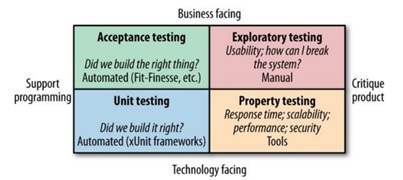
\includegraphics[width=1\textwidth]{test_types.jpg}
    \caption{Rodzaje testów. Źródło: \cite{newman2015}}
    \label{fig:test-types}
\end{figure}

Dwie kategorie znajdujące się na dole - \textit{unit testing} oraz \textit{property testing} - mają 
pomóc deweloperom utworzyć działający kod. Tego rodzaju testy mają na celu 
sprawdzenie, czy system nie jest obciążony usterkami związanymi z implementacją. 
Celem testów należących do dwóch kategorii znajdujących się na górze - \textit{acceptance 
testing} oraz \textit{exploratory testing} - jest pomoc w zrozumieniu jak dany system działa. 
Do tego rodzaju testów można zaliczyć m. in. szerokie testy obejmujące działanie dużej 
liczby mikroserwisów, sprawdzenie funkcjonalności systemu oraz tzw. \textit{user acceptance 
testing}, czyli testy przeprowadzone przez klienta, który zlecił budowę systemu.

\subsection{Testy jednostkowe}

Tego rodzaju testy sprawdzają poprawność pojedynczej metody w kodzie. Nie sprawdza się działania 
się całego mikroserwisu, a jedynie jego wyodrębioną część. Wszystkie parametry, które 
przyjmuje dana funkcja, są tworzone w trakcie testu. Testy jednostkowe są wykonywane 
w pierwszej fazie testów ze względu na szybkość ich wykonania. Ich celem jest wykrycie 
błędów związanych z daną technologią, nie zaś sprawdzenie, czy działanie systemu jest 
zgodne z oczekiwaniami klienta. Należy zapewnić dużą liczbę testów 
jednostkowych, ponieważ jest to najszybszy sposób zlokalizowania potencjalnych awarii.

Przykładem jest poniższy test:

\begin{lstlisting}
    [Test]
    public void MeasurementsTooHighIndicatorsTest()
    {
        // Arrange
        var currentMeasurement = 
        CreateMeasurementSentEvent();
        var policy = TestPoliciesDataService
            .CreateNewRoomPolicyDto(
                15, 80, 0.3f, 2, 20, 0.1f);

        // Run
        var result = 
        _policyEvaluator!
            .Evaluate(currentMeasurement, policy);
        
        // Assert
        Assert.AreEqual(
            result.TemperatureStatus, 
            EvaluatorResult.TooHigh);
        Assert.AreEqual(
            result.IlluminanceStatus, 
            EvaluatorResult.TooHigh);
        Assert.AreEqual(
            result.HumidityStatus, EvaluatorResult.TooHigh);
    }
\end{lstlisting}

Sprawdza on działanie logiki odpowiedzialnej za porównanie aktualnie panujących 
warunków w pomieszczeniu z warunkami oczekiwanymi. Test składa się z trzech części:

\begin{itemize} % lista nienumerowana
    \item Arrange - przygotowanie niezbędnych komponentów potrzebnych do przetestowania 
    fragmentu kodu
    \item Run - faktyczne uruchomienie testowanego kodu
    \item Assert - sprawdzenie otrzymanego wyniku z oczekiwanym rezultatem
\end{itemize}

\subsection{Testy integracyjne}

Testy integracyjne mają na celu sprawdzenie, czy poszczególne mikroserwisy będą 
w stanie się ze sobą skutecznie komunikować. Przykładem jest poniższy test:

\begin{lstlisting}
    [Test]
    public async Task 
    GetExpectedRoomConditionsAvailabilityTest()
    {
        var path = 
        $"policies-api/expected-room-conditions/1";
    
        var response = await _client.GetAsync(path);
    
        response.StatusCode.Should().Be(HttpStatusCode.OK);
    }    
\end{lstlisting}

Klient testowy korzysta z oferowanej przez testowany mikroserwis usługę poprzez 
wysłanie żądania http. W tym przypadku nie jest testowana logika zawarta w testowanym 
mikroserwisie, a jedynie odpowiedź, którą odsyła. Status odpowiedzi powinien oznaczać 
sukces, sygnalizowany przez kod 200 OK \cite{fielding1999}.

\subsection{Testy end-2-end}

Testy typu end-2-end mają za zadanie przetestować pewne biznesowe 
funkcjonalności, których realizacja może być obsługiwana przez wiele mikroserwisów. 
Dobrą praktyką jest utrzymywanie niewielkiej liczby tego typu testów, ponieważ 
obejmują one zakres działania całego systemu i przeprowadzenie każdego z nich zajmuje dużo 
czasu. Ponadto, w przypadku wystąpienia usterki ciężko jest wykryć miejsce, które 
było źródłem błędu.
Przykładem jest poniższy test, napisany w języku programowania Python:

\begin{lstlisting}
def measurement_triggers_policies_evaluation_result_event():
    new_measurement_test_helper = NewMeasurementTestHelper()

    new_measurement_test_helper
        .check_influxdb_is_available()

    new_measurement_test_helper
        .check_sensors_api_is_available()

    new_measurement_test_helper
        .send_new_measurement_to_rabbitmq()

    new_measurement_test_helper
    .check_message_sent_to_queue(
        new_measurement_test_helper
        .rabbitmq_configuration.vhost,
        consts.sensors_test_queue, 
        1)

    new_measurement_test_helper.
    check_message_sent_to_queue(
        new_measurement_test_helper
        .rabbitmq_configuration.vhost,
        consts.measurement_sent_event_test_queue, 
        1)

    new_measurement_test_helper.
    check_message_sent_to_queue(
        new_measurement_test_helper
        .rabbitmq_configuration.vhost,
        consts.policies_evaluation_result_event_test_queue, 
        1)
\end{lstlisting}

W tym teście sprawdza się odpowiedź całego systemu na otrzymanie nowego pomiaru 
z sensora. Jako skutek powinna zostać wygenerowana odpowiednia wiadomość z wynikiem 
przetworzenia pomiaru, która została wysłana na kolejkę wiadomości.

\subsection{Automatyzacja testów}

Ręczne uruchamianie każdego z testów pojedynczo może szybko stać się żmudnym zajęciem. 
Aby temu zaradzić, w ramach pracy inżynierskiej wykorzystano narzędzie do automatyzacji 
o nazwie Nuke \cite{nuke2022}. 
Za jego pomocą uruchomienie wszystkich testów sprowadza się do wykonania 
jednej komendy. 

Nuke pozwala na tworzenie własnych metod zwanych zamiarami (ang. \textit{target}), które automatyzują 
wykonywanie pewnych czynności. Każdy z zamiarów wykonuje określoną logikę. 
Dodatkowo, można tworzyć kompleksową strukturę, w której każdy z zamiarów jest zależny 
od tego, czy prawidłowo zostanie wykonany inny. Istnieje także możliwość 
dodania reguły wyzwalania poszczególnych zamiarów po wykonaniu innego. 
Przykładowo, metoda uruchamiająca test dla konkretnego projektu wygląda w sposób 
następujący:

\begin{lstlisting}
Target TestProject => _ => _
.DependsOn(CompileTestProject)
.Executes(() =>
{
    var solution = (this as IHaveSolution).Solution;
    var project = solution
        .AllProjects
        .Single(x => 
        x.Name == TestProjectNames[ProjectName]);
    DotNet($"test {project} --no-build -c {Configuration}");
});
\end{lstlisting}

Wykonuje ona metodę \textit{dotnet test}, uruchamianą dla konkretnego projektu. 
Wykonanie zamiaru zależy od pomyślnego wykonania innego, o nazwie \textit{CompileTestProject}.

\begin{lstlisting}
Target CompileTestProject => _ => _
.DependsOn(RestoreTestProject)
.Executes(() =>
{
    var solution = (this as IHaveSolution).Solution;
    var project = solution
        .AllProjects
        .Single(x => 
        x.Name == TestProjectNames[ProjectName]);
    DotNetBuild(s => s
        .EnsureNotNull(
            this as IHaveSolution, (_, o) => 
            s.SetProjectFile(project))
        .SetConfiguration(Configuration)
        .EnableNoRestore());
});
\end{lstlisting}

Metoda wykonuję komendę \textit{dotnet build}. Jest ona 
zależna od zamiaru \textit{RestoreTestProject}.

\begin{lstlisting}
Target RestoreTestProject => _ => _
.DependsOn(Clean)
.Requires(() => ProjectName)
.Executes(() =>
{
    var solution = (this as IHaveSolution).Solution;
    foreach (var proj in solution.AllProjects)
    {
        Logger.Info(proj.Name);
    }
    var project = solution
        .AllProjects
        .Single(x => 
        x.Name == TestProjectNames[ProjectName]);
    DotNetRestore(s => 
    s.EnsureNotNull(
        this as IHaveSolution, (_, o) => 
        s.SetProjectFile(project)));
});
\end{lstlisting}

Metoda wykonuje funkcję \textit{dotnet restore}. Jednym z 
warunków uruchomienia tego zamiaru jest konieczność podania nazwy projektu, wyrażona 
przez funkcję \textit{.Requires(() => ProjectName)}. Uruchomienie zamiaru jest zależne od poprawnego
wykonania innego, o nazwie \textit{Clean}.

\begin{lstlisting}
Target Clean => _ => _
.Executes(() =>
{
    SourceDirectory
    .GlobDirectories("**/bin", "**/obj")
    .ForEach(DeleteDirectory);
    EnsureCleanDirectory(ArtifactsDirectory);
});
\end{lstlisting}

Metoda czyści repozytorium z artefaktów. Nie jest zależna od żadnego innego zamiaru.
Wszystkie zamiary można uruchomić jednocześnie przy pomocy jednej metody:

\begin{lstlisting}
./build.sh TestProject --ProjectName facilities 
    --verbosity verbose
\end{lstlisting}